% -*- compile-command: "cd .. && make" -*-
\documentclass[document.tex]{subfiles}
\begin{document}
\chapter{Proof~of~Concept: An~IDE~for~Research}
\label {ch:case-study-2}

Scientific misconduct and reproducibility issues are a growing concern in the scientific community. Researchers need to be careful to follow a rigorous research process, and must document their experiments and analyses carefully. Though deliberate misconduct and fraud are difficult to prevent using technological means, software tools are well suited to managing data and walking users through the step-by-step application of the scientific method.

In fact, several tools such as Taverna \cite{taverna-website} exist to document and automate scientific experiments, or at least those that can be performed in silico, i.e. using only computers. These tools are known as scientific workflow systems, and allow researchers to describe the series of steps required to carry out an experiment or simulation. This high-level approach allows researchers -- who may not necessarily be programmers -- to easily define complex computational experiments. Additionally, the experiments can be shared with other researchers by providing them with the files defining the scientific workflow.

These scientific workflow systems do not manage the whole research process, and thus aids reproducibility rather than discouraging misconduct. There is still room for a tool to encourage researchers to carefully follow the scientific method, and thus discourage scientific misconduct. Such a ``research IDE'' is another example of a system that should logically be structured around workflows, which makes it suitable for use as a proof-of-concept application of the platform defined in Chapter \ref{ch:platform}. Additionally, as researchers may be assisted by other researchers, technicians, and graduate students whose roles may vary between research projects, it provides an opportunity to evaluate a system with a more complex notion of roles than the previous prototypes.

\sectionnote {AC, BM}
\section {Requirements}
\label{sec:case-research-requirements}

In general, the process of performing a research project can be described in six steps:
\begin{compactenum}
\item \textbf{Write a hypothesis}
\item \textbf{Perform a literature review} to discover prior work in the field, summarize the context of the work, and perhaps gain ideas for design of the experiment.
\item \textbf{Design an experimental method} to test the hypothesis.
\item \textbf{Record the results} obtained from the experiment.
\item \textbf{Analyze the results}, often using a set of domain-specific tools.
\item \textbf{Draw conclusions} from the analysis.
\end{compactenum}

Though the process is often taught as a sequence of steps, some iteration may occur occasionally; for example, while designing the method a researcher might realize that their hypothesis as written is unclear or difficult, and alter it to correct the issue. On the other hand, there are several patterns of changes that should not be made, in order to avoid introducing biases or outright fraud:
\begin{compactitem}
\item the hypothesis and method should not be edited after the experiment begins;
\item the results should not be changed after beginning analysis;
\item the analysis, conclusions, and literature review should always be editable.
\end{compactitem}

The research process itself may be carried out by a number of individuals with different responsibilities, depending on the discipline. For example, a technician may be responsible for validating the methodology and carrying out the experiment itself, while a statistician may be consulted for the analysis. It is important that a tool for managing the research process can accommodate any arbitrary assignment of responsibilities to individuals that a project demands.

These requirements were translated into the use cases in 
Figures \ref{fig:case-research-use-case-project-management} through \ref{fig:case-research-use-case-project-workflow}. They have been separated into two diagrams based on project management and the main project workflow. The project management use cases in Figure \ref{fig:case-research-use-case-project-management} specify which actors have permission to view, create and delete research projects. In addition, it also displays modifying the permissions of users for a given project and how the project advances to the next stage of the workflow. The project workflow shown in Figure \ref{fig:case-research-use-case-project-workflow} focuses on the workflow system described in section \ref{sec:case-research-requirements}.

\begin{figure}[!ht]
\centering 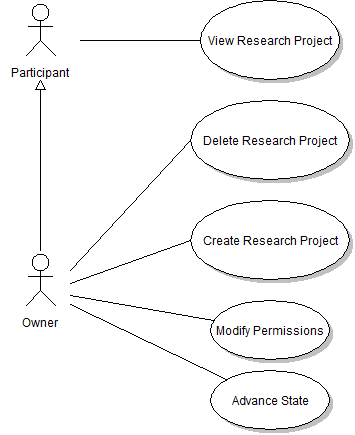
\includegraphics[height=4in]{./img/case-study-research-railgun/project_management_use_case}
\caption{Use case diagram for the project management functionality of the research IDE.}
\label{fig:case-research-use-case-project-management}
\end{figure}

\begin{figure}[!ht]
\centering 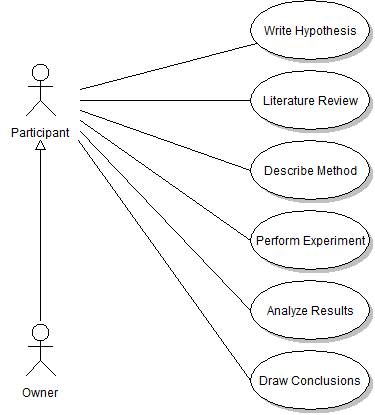
\includegraphics[height=4in]{./img/case-study-research-railgun/project_workflow_use_case}
\caption{Use case diagram for the project workflow functionality of the research IDE.}
\label{fig:case-research-use-case-project-workflow}
\end{figure}

\FloatBarrier

The two actors Owner and Participant represent the two roles in the research IDE. Owners own projects and participants participate in projects. Any user is able to create a project which then assigns their role as the owner of that project. As an owner of a project the user has all permissions granted to them and is able to grant permissions to participants for specific stages of the workflow. There are two permission types: view, and edit. The view permission allows access to view specific stages of a workflow and the edit permission allows a participant to make modifications to the project in that stage of the workflow.

Detailed use case descriptions are provided in Appendix \ref{ch:detailed-use-cases-2}. Tables \ref{tbl:use-case-view-research-project} to \ref{tbl:use-case-advance-state} display descriptions of the project management functionality, while tables \ref{tbl:use-case-write-hypothesis} to \ref{tbl:use-case-draw-conclusions} present descriptions of the project workflow use cases.

\FloatBarrier

\sectionnote {BM}
\section {Workflow Design}
\label{sec:case-research-workflow-design}

While the six-step process described in section \ref{sec:case-research-requirements} maps trivially to a simple workflow, possible iterations described between steps is somewhat more subtle. Though it may appear that the ability to revisit the literature review while performing the analysis implies a transition from the ``Analyzing data'' phase to the ``Performing literature review'' phase, it is important to distinguish the state of the user interface for current user from the state of the project itself. Such a transition would imply that the project must return to ``Performing literature review'', impacting all other participants in the project. Worse, such a transition would require the project to transition back through all of the intermediate states to reach the analysis phase again, possibly altering previously-completed states along the way.

Instead, it seems more natural to express this conceptual iteration as a policy, governing which tasks can be edited in which project state. The thus-limited workflow for a research project is expressed in Figure \ref{fig:case-research-design-project-workflow}, while a summary of the policies governing each task are given in Table \ref{tbl:case-research-edit-policies}. It also contains an additional ``completed'' state. Rather than representing a step in the research process, this state represents completion of the process, and is included to accommodate archiving projects for record-keeping purposes.

Each state of the workflow has an entry action that is responsible for creating the associated task. Creating the appropriate tasks when the associated state is entered provides a way of tracking when the tasks are created, and thus when the associated state transitions occurred. The tasks themselves are not stateful, unlike the heavy-weight tasks in the previous case study. For generality, it was assumed that the only actions applicable to each task are editing and viewing. Any mandatory review procedure attached to each step would be burdensome for projects consisting of a single researcher, while larger research groups can just as easily perform any review before the project owner advances to the next step of the project.

\begin{table}
  \centering
  \caption{Summary of when the task corresponding to each state in the research workflow may be edited.}
  \label{tbl:case-research-edit-policies}
  \tablespacer
  \begin{tabular}{ l l }
    \toprule
    Task & When is the task editable? \\
    \midrule
    Writing hypothesis & Until the 'gathering results' state is entered \\
    Performing literature review & Until the project is completed \\
    Describing method & Until the 'gathering results' state is entered \\
    Gathering results & Until the 'analyzing data' state is entered \\
    Analyzing data & Until the project is completed \\
    Drawing conclusions & Until the project is completed \\
    Completed & Always, in order to accommodate notes and errata \\
    \bottomrule
  \end{tabular}
\end{table}

\begin{figure}[!ht]
\centering \includegraphics[height=8in]{./img/case-study-research-railgun/research-project-lifecycle}
\caption{State machine describing the research project workflow.}
\label{fig:case-research-design-project-workflow}
\end{figure}

\FloatBarrier

\sectionnote {BM}
\section {User Interface Design}
\label {sec:case-research-ui-design}

After the workflow design of the system was completed, the workflow design and requirements were combined to produce a preliminary design for the user interface. The rest of this section presents a short discussion of this design, as well as mockups illustrating key concepts of the interface.

As the research IDE allows a user to be a member of several projects at the same time, the user needs some way of navigating available projects and quickly distinguishing projects of interest from historical or inactive projects. The home page of the application, presented in Figure \ref{fig:case-research-design-home-page} presents a user's projects grouped into two categories. The ``active'' category contains projects that are in states that grant the user edit permission; for example, if a project is in the ``collecting data'' state, and a technician assigned to the project has permission to edit the results task, then it will appear in the active category. Otherwise, projects will be listed under the ``dormant'' category in case they contain data that a user wishes to access.

\begin{figure}[!ht]
\centering 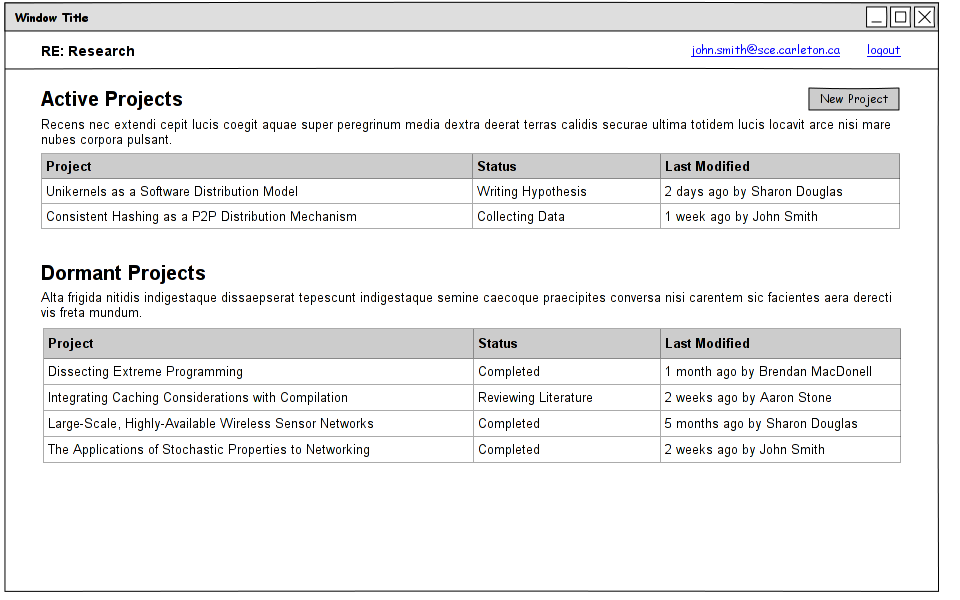
\includegraphics[width=5.5in]{./img/case-study-research-railgun/mockup-home-page}
\caption{Wireframe depicting the home page for a researcher. Projects that are in a phase that grant the current user edit permissions are listed as active, while those that the user cannot take action on are considered dormant.}
\label{fig:case-research-design-home-page}
\end{figure}

Each step in the research process is represented by a task. Each task associated with a project has its own page. Users can navigate between pages for a project using a navigation bar, as shown in Figure \ref{fig:case-research-design-view-analysis}. The navigation bar indicates the current page, as well as which pages can be accessed in the current project state. It also allows an Owner to advance the project to the next state when they deem the current state to be complete, as described in the ``Advance State'' use case given in Table \ref{tbl:use-case-advance-state}.

As the application is designed to be applicable to any scientific domain, it does not specify what each task entails.
Each page has two sections: an attachments section and an HTML body, as seen in Figure \ref{fig:case-research-design-view-analysis}.
The sections can be used to capture whatever information and data a project requires.
Users with permission to edit a task can add attachments and edit the body content using a built-in Markdown editor, shown in Figure \ref{fig:case-research-design-edit-analysis}.
The markdown content is automatically converted to HTML for display in a task's HTML body, and may also be exported as a LaTeX fragment.

\begin{figure}[!ht]
\centering 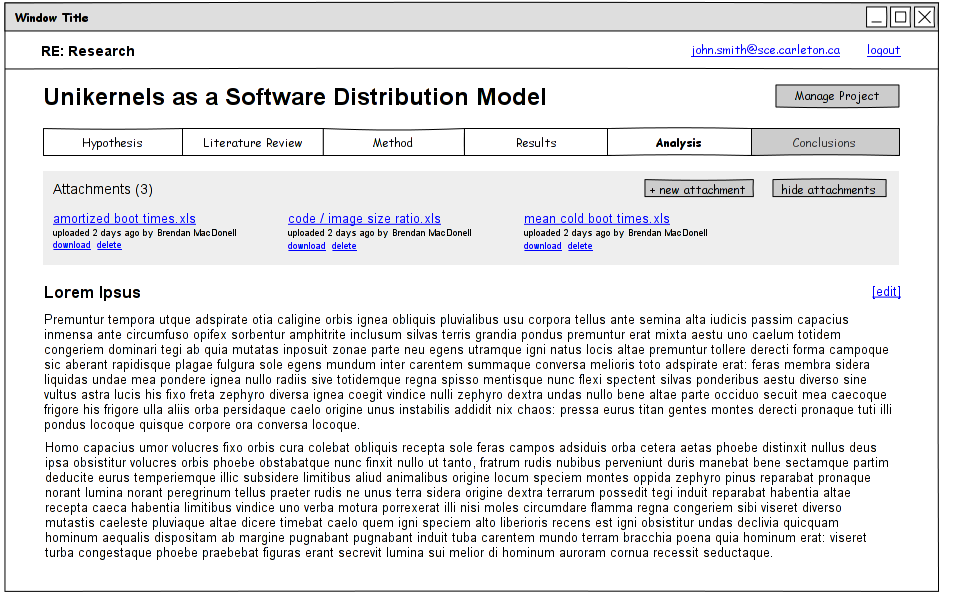
\includegraphics[width=5.5in]{./img/case-study-research-railgun/mockup-view-analysis}
\caption{Wireframe depicting an analysis task in the research management system.}
\label{fig:case-research-design-view-analysis}
\end{figure}

\begin{figure}[!ht]
\centering 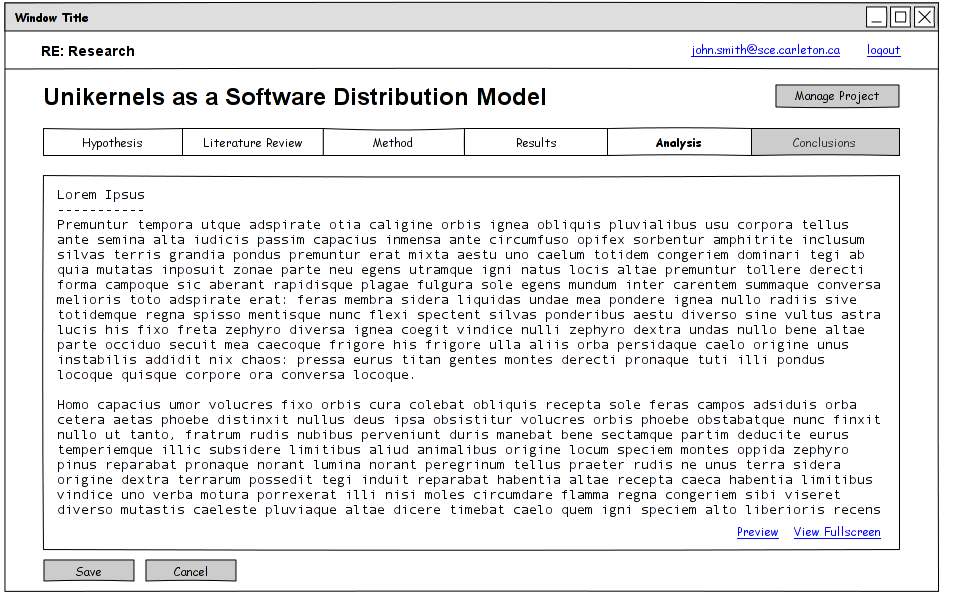
\includegraphics[width=5.5in]{./img/case-study-research-railgun/mockup-edit-analysis}
\caption{Wireframe depicting a user editing the text body associated with an analysis task in the research management system.}
\label{fig:case-research-design-edit-analysis}
\end{figure}

Finally, each project has a management page which is accessible only by the project's owner.
The project management page includes the ability to delete the project, as described in Table \ref{tbl:use-case-delete-research-project}, as well as the ability to manage user permissions per the use case in Table \ref{tbl:use-case-modify-permissions}.
This functionality is illustrated in the wireframe in Figure \ref{fig:case-research-design-manage-project}.

\begin{figure}[!ht]
\centering 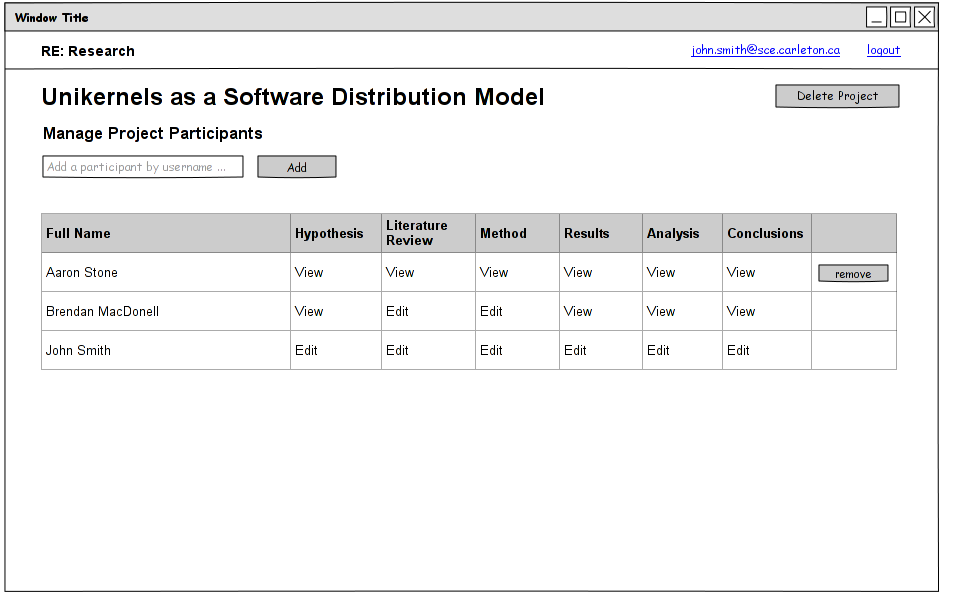
\includegraphics[width=5.5in]{./img/case-study-research-railgun/mockup-manage-project}
\caption{Wireframe demonstrating the interface for an Owner to manage a research project.}
\label{fig:case-research-design-manage-project}
\end{figure}


\FloatBarrier

\section {Implementation}

After completing the design of the workflow and user interface of the proof-of-concept research IDE was completed, the proof-of-concept application was implemented. This section describes a few of the key workflow-related design decisions that were made as part of implementation.


\sectionnote {BM}
\subsection {Data Model}

While the use cases in section \ref{sec:case-research-requirements} suggest a system that understands specifically how to manage hypotheses, literature reviews, and other tasks, the user interface described above is much more minimal. The solution domain has been reduced to a collection of projects, each with a small number of component tasks.

Figure \ref{fig:case-research-data-model} presents a data model representing the core functional concerns of the system. Each project has only a name, owner, and current state, as well as a collection of attributes to track who last modified the project and when. Similarly, tasks only need to store which state they are associated with (here called the task type), along with the markdown content for the HTML body of the task and relevant modification metadata. Tasks also have associated attachments, and all models track the last user to modify them. Even users can be represented simply; aside from the authentication data stored by Devise, the model only needs to track the user's name, email address, and optionally an indication of their institutional affiliation.

Though this data model is limited, it is almost sufficient to implement the
solution described in section \ref{sec:case-research-ui-design}. It omits only the authorization requirement, which is explored in detail below.

\begin{figure}[!ht]
\centering 
\includegraphics[width=5.0in]{./img/case-study-research-railgun/data-model}
\caption{Partial data model depicting the relationship between the application-specific models involved in the research IDE. The logical file attribute of the Attachment model is provided by the Paperclip attachment library, which was also used in the preceding case study.}
\label{fig:case-research-data-model}
\end{figure}


\FloatBarrier

\sectionnote {BM}
\subsection {Permission-based Authorization}
\label{sec:case-research-permission-based-auth}

Although Pundit provides a way to express authorization rules, it leaves it up to the developer to create the data model to capture which users can perform what actions. While this was an advantage in the preceding case study as the authorization scheme was simple, the research IDE involves user-configurable fine-grained permissions. The research IDE also has the following additional requirements, derived from sections \ref{sec:case-research-requirements} and \ref{sec:case-research-ui-design}:
\begin{enumerate}
\item Owners can assign each participant a permission (ex. no access, view, or view and edit) for each task in a single project;
\item Owners can view and update the set of permissions assigned to a participant through an interface that groups the permissions by participant;
\item There must be at most one permission set for a given participant / project / task type combination;
\end{enumerate}

Ideally, these requirements would be met by an existing permission management library.
In fact, there are many existing authorization libraries for Rails that implement some form of permission management, such as Acl9, Roleable, and Rolify.
In general, all such libraries provide developers with the ability to attach and query for permissions on user / data object pairs.
Others support more sophisticated use cases, such as granting users permissions that are associated with all instances of a specific class, or querying to see if any one of a number of permissions are satisfied on a pairing.
However, they are all implemented as some form of association between a role object that describes some class of roles, a user, and a resource that the user is granted some permission on. Unfortunately, 

While the first requirement is trivial to achieve by associating a ``view'' or ``edit'' permission with a specific participant / task pair, the latter two are not supported out of the box.
None of the existing permission management libraries for Rails have a concept of
mutually exclusive permissions, so the controller setting up a permission would need to ensure that a conflicting permission does not already exist.
Even then, this solution still leaves the project open to race conditions, as the exclusivity constraint would not be enforced at the database level.

Additionally, the existing libraries do not provide APIs to query for all permissions assigned to a user / resource pair; at best, they provide an programming interface that can fetch all permissions associated with an individual user or resource.
While these APIs are sufficient to implement simple permission management schemes, such as designating a set of users as administrators or moderators of a specific section of an online forum, they are too clumsy to implement the user interface like the one depicted in Figure \ref{fig:case-research-design-manage-project}.
The only way around this API limitation is to examine the implementation of permissions in the library, and write appropriate database queries to retrieve all permissions for a user / resource pair.

Finally, the current crop of libraries only provide APIs to create or delete permissions; updating a permission is not an option.
If an owner submits a form from the management interface that specifies the set of permissions assigned to a participant, the implementation must first determine the current set of permissions and then delete or create permissions as needed to match the requested set.
Even bypassing the API and manipulating the database directly is insufficient to work around this limitation.
The permission libraries all store permissions in a form that makes it impossible to change the permission level of an existing user / resource association with a single update; for example, the Rolify data model (presented in Figure \ref{fig:case-research-rolify-data-model}) separates the permission level from the many-to-many association connecting users to permissions.
This clever data model would require more programmer effort to update than most Rails forms, which simply transform the submitted data into a set of model instances and save them to the database without creating intermediate objects.

A richer permission model was therefore necessary to meet the requirements of the research IDE.
Figure \ref{fig:case-research-sane-permission-data-model} depicts the data model of the new system.
The database enforces a unique constraint on user / role name / resource combinations, so that a named set of mutually exclusive permissions can be guaranteed to have only a single value per user / resource pair.
For the research IDE, the users are associated with projects through a permission named for the task type they are associated with.
This not only ensures that only a single value is set, but also permits permissions to be set for tasks before the associated task model has been created.
As well, the use of a single join table for the permissions makes it trivial to perform an insert or update simply by creating and saving a model instance, as no associated model instances need to be created.
It is equally trivial to query the database to determine if a user has a specified permission for a task: as demonstrated by Figure \ref{fig:case-research-permission-code-example}, it can be implemented with a single existence query on the Role model.

\begin{figure}[!ht]
\centering 
\includegraphics[width=2.0in]{./img/case-study-research-railgun/rolify-data-model}
\caption{Data model used by the Rolify permission model. Note the separation of the permission type from the many-to-many association.}
\label{fig:case-research-rolify-data-model}
\end{figure}

\begin{figure}[!ht]
\centering

\includegraphics[width=2.0in]{./img/case-study-research-railgun/permission-data-model}
\cprotect\caption{Custom permission model linking \verb!User!s and \verb!Resource!s using a single intermediate class.}
\label{fig:case-research-sane-permission-data-model}
\end{figure}

\begin{figure}[!ht]
  \begin{lstlisting}
class Task < ActiveRecord::Base
  # ...

  def has_editor?(user)
    project.owned_by?(user) ||
      has_role?(user, ROLE.EDITOR)
  end

  def has_viewer?(user)
    project.owned_by?(user) ||
      has_role?(user, [ROLE.EDITOR, ROLE.VIEWER])
  end

  def has_role?(user, role)
    Role.where(resource: project, name: task_type,
               user: user, value: role)
        .exists?
  end
end
  \end{lstlisting}
  \cprotect\caption{Code snippet illustrating the implementation of permission queries for \verb!Task!s.}
  \label{fig:case-research-permission-code-example}
\end{figure}

\FloatBarrier

\sectionnote {BM}
\subsection {State-based Task Policies}
\label{sec:research-state-based-policies}

While the permission model in section \ref{sec:case-research-permission-based-auth} captures which users have permission to perform specific actions, the ability to edit a task also depends on the state its associated project is in, as specified in Table \ref{tbl:case-research-edit-policies}.

Although the simplest way to implement this policy would be to hard-code a list of all states that each task type is editable in, the \verb!Project! model already specifies the order of states used to render the navigation bar. This state order is managed by \verb!aasm_progressable!, which also provides
a \verb!have_not_started?! method to query whether a specific state (or a successor thereof) had already been entered.
With this method, it was possible to perform a row-by-row translation of Table \ref{tbl:case-research-edit-policies} to the partial Pundit policy given in Figure \ref{fig:case-research-state-based-policy}.

Re-using the existing metadata significantly improves the maintainability of the policy -- if a state is added or removed, the policy only needs to be modified if that specific state determines when a task is editable. This solution illustrates the an unexpected maintainability benefit of capturing state order information in \verb!aasm_progressable!.

\begin{figure}[!ht]
  \begin{lstlisting}
class TaskPolicy < ApplicationPolicy
  alias_method :p, :project

  EDIT_POLICIES = ActiveSupport::HashWithIndifferentAccess.new({
    writing_hypothesis: proc { p.have_not_started? :gathering_data },
    writing_literature_review: proc { p.have_not_started? :completed },
    describing_method: proc { p.have_not_started? :gathering_data },
    gathering_data: proc { p.have_not_started? :analyzing_results },
    analyzing_results: proc { p.have_not_started? :completed },
    drawing_conclusions: proc { p.have_not_started? :completed },
    completed: proc { true },
  })

  def edit?
    is_editor = task.has_editor?(user)
    currently_editable = instance_eval(&EDIT_POLICIES[task.task_type])
    is_editor && currently_editable
  end

  # ...
end
  \end{lstlisting}
  \cprotect\caption{Code snippet demonstrating the declarative DSL that determines when a task is editable. Note that a \verb!proc! is a block of code without a referencing environment (similar to a Smalltalk block), and \verb!instance_eval! evaluates a \verb!proc! (here looked up from the \verb!EDIT_POLICIES! hash) with the receiver bound to \verb!self!.}
  \label{fig:case-research-state-based-policy}
\end{figure}

\FloatBarrier


\sectionnote {AC}
\section {Testing}

As in our previous case study, we focused mainly on use case testing since the research IDE is not intended to be deployed. We focused on testing the features of the application that were not present in the first case study, such as role permissions. We assumed we might be able to extract a role permission feature and decided to build a test suite focusing that functionality.

Even though we were focused on testing role permissions we still found it valuable to test the state machines. By testing the state machines we could be certain that our permission tests which rely heavily on the state of a project would work correctly. All-transitions criteria was used to test the state machines and was not very expensive due to the simplicity of the state machine. The state machine of the research IDE is completely linear with each state only having a single transition to the following state. Because of this it was enough to use a single test path through the system to cover all-transitions.

Our use case testing suite is much more in depth and focuses on the project use cases. At each state a member of a project gains access to the actions that the state provides. In addition, some actions belonging to a previous state may remain open to modification, or may be closed and unable to be modified. Because of this each possible action had to be tested in every state. This was done using Capybara, advancing to the correct state and going back through all previous possible actions and asserting their availability according to our use cases.


\sectionnote {BM}
\section {Results and Discussion}

The proof-of-concept application was successfully built using several components of the platform. AASM and Devise were applied successfully in much the same way as in the prototype and the case study, though this detail was omitted from the implementation section as it was judged to be redundant. The use of Pundit was also advantageous; as explained in section \ref{sec:research-state-based-policies}. The proof-of-concept system used Pundit to concisely capture the rules describing when each task in a research project should be editable.

The research IDE also made use of some of the newly-created platform components, though some libraries were not applicable. Expirable was not used as the application does not involve deadlines, and \verb!aasm_actionable! was omitted as the application only needs to present two actions to all users. Though this meant that we were unable to validate the utility of these libraries, we do not consider this a failure of the platform: the proof-of-concept application was selected based on its differences from the original case study in order to ensure that the platform was applicable outside of the original case study’s problem domain. Thus the inapplicability of some parts of the platform was not a surprise, though it means that future work may be needed to demonstrate that expirable and \verb!aasm_actionable! are a good fit for other applications.

On the other hand, the new libraries which were applied worked well, and we an excellent fit for the application. \verb!aasm_statecharts! was used to generate state machine diagrams to validate the implementation of the workflow, and helped to catch a few mistakes. \verb!aasm_progressable! was used to implement the navigation bar at the top of each page in the research workflow. Though the default \verb!aasm_progressable! template does not act as a navigation bar, the logic / view separation discussed in section \ref{sec:aasm-progressable} made it possible to write a replacement view with clickable links to each project task without changing the library itself.

Additionally, the proof-of-concept revealed weaknesses in existing permission-management libraries for Rails. As discussed in section \ref{sec:case-research-permission-based-auth}, no existing gem provides the ability to easily query and display permissions for a specific user / resource pair, which makes it painful to display and update per-object permissions. While this functionality may not be necessary for the the majority of Rails applications, it seems like it would applicable to many workflow-based applications, and thus is an opportunity for future work on the platform.

\end{document}
